\section{Resultat}
todo

\subsection{Parser} 
%TODO

\subsection{Abstrakt syntaxträd} 
%TODO

\subsection{Typcheckare} 
%TODO


\subsection{HIJi}


HIJi erbjuder användaren ett GHCi-liknande gränssnitt. HIJi fungerar som en fasad in i programmet. 
HIJi tar input genom att användaren skriver in Haskellkod som därefter tolkas av parsern och slutligen evalueras uttrycket. Resultatet av uttrycket visas på raden under.

HIJi är skapat för att likna GHCi i så stor utsträckning som möjligt. Det finns väldigt goda anledningar till att göra detta. Dels är GHCi ett mycket kompetent verktyg när man programmerar i Haskell. Att kolla upp funktionsdeklarationer och testa kodfragment är något som varje professionell haskellprogrammerare gör varje dag. Genom att efterlikna GHCi så kommer användare känna igen sig när de tar steget från HIJi till GHCi. Det blir för dem ett naturligt steg och kortar inlärningströskeln avsevärt. Även för haskellprogrammerare som är väl införstådda i GHCi's möjligheter blir det lättare att använda sig utav HIJi, de behöver inte fundera hur verktyget ska användas.
% Dock finns det vissa nackdelar med ett terminalliknande gränssnitt. 

\begin{figure}
    \begin{center}
        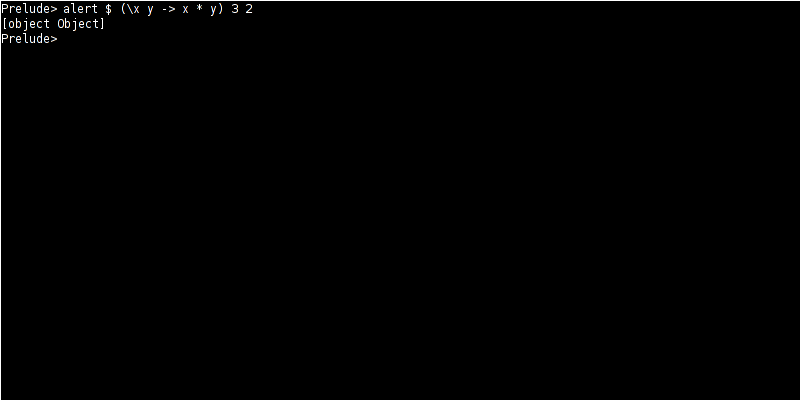
\includegraphics[width=1\textwidth]{hiji_screen3.png}
        \caption{HIJi användargränssnitt}
    \end{center}
\end{figure}

%Byt ut denna bilden om hiji uppdateras!
Bilden ovan visar hur HIJi ser ut för användaren. De första raderna visar precis som i GHCi vilka moduler som för närvarande är laddade. I detta exemplet är det en modul laddad med namnet Prelude. Därefter följer en prompt där användaren fritt kan skriva in egna funktioner. I exemplet har användaren använt sig utav en av de inbyggda funktionerna i Prelude och en lambda-funktion.

%TODO get source from cp-book at home

HIJi är tänkt att erbjuda användaren liknande möjligheter som GHCi. 

% TODO skriv om detta
Fördelen med HIJi framför GHCi är att användaren ej behöver ladda ner den tunga GHC-kompilatorn på sin personliga dator för att testa enkla Haskelluttryck direkt i webbläsaren.
Nackdelar gentemot GHCI är att HIJi är en nedbandat version utav GHCi. HIJi kan bara evaluera enklare uttryck. Det finns i dagsläget inga möjligheter att ladda upp hela Haskell-filer för att köra dem. Att som i GHCi på ett enkelt sätt kolla upp vilka typer en funktion stöds ej.

Ett stort problem för alla webbutvecklare idag är att de idag marknadsledande webbläsarna tolkar Javascript på olika sätt. Det har därför kommit fram en rad olika kodbibliotek för att lösa detta problemet. Ett av dessa är JQuery som HIJi använder sig utav för att få ett unisont stöd på alla moderna webbläsare. 


